\chapter{Development}

\section{Experiment Design}
The following section explains how the different experiments were conducted in detail. Further, it is shown how the datasets and anomalies were engineered.

\subsection{Experiment 1}
The first experiment was conducted on a fully synthetic dataset. Supervised and unsupervised learning approaches were used to detect the anomalies. 

\subsubsection{Dataset}
The dataset, that was created for this first task consisted of five variables. The dataset was created under the assumption, that one measurement was drawn per hour on totally 2000 days, resulting in 48000 datapoints. The variables all follow a cyclic pattern shown in figure \ref{fig:synthetic data}. 

\begin{figure}[h]
	\centering
	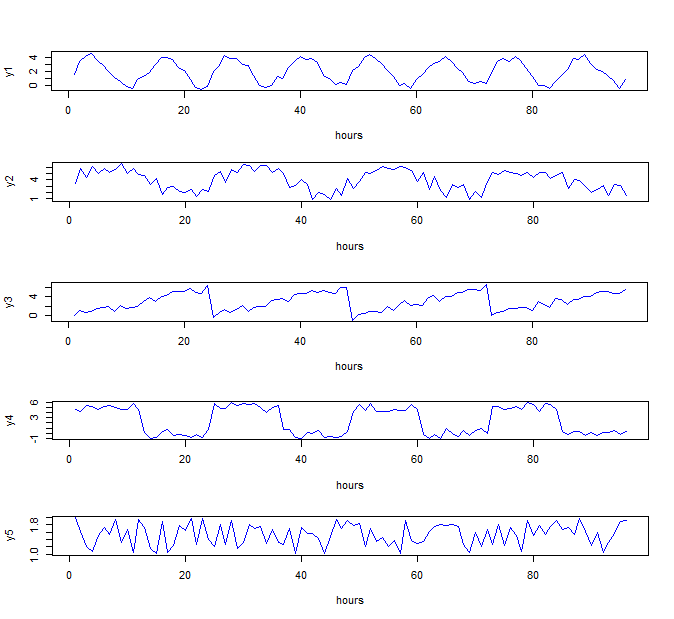
\includegraphics[scale=0.6]{Figures/synthetic data}
	\decoRule
	\caption[Synthetic Dataset]{Synthetic Dataset \parencite{own}}
	\label{fig:synthetic data}
\end{figure}

In a second step the dataset was enriched with six different kinds of anomalies. The anomalies embedded into the dataset are of type deviant cycle, temporary change and level shift. Figure \ref{fig:anomalies} shows examples of the embedded anomalies.

\begin{figure}[h]
	\centering
	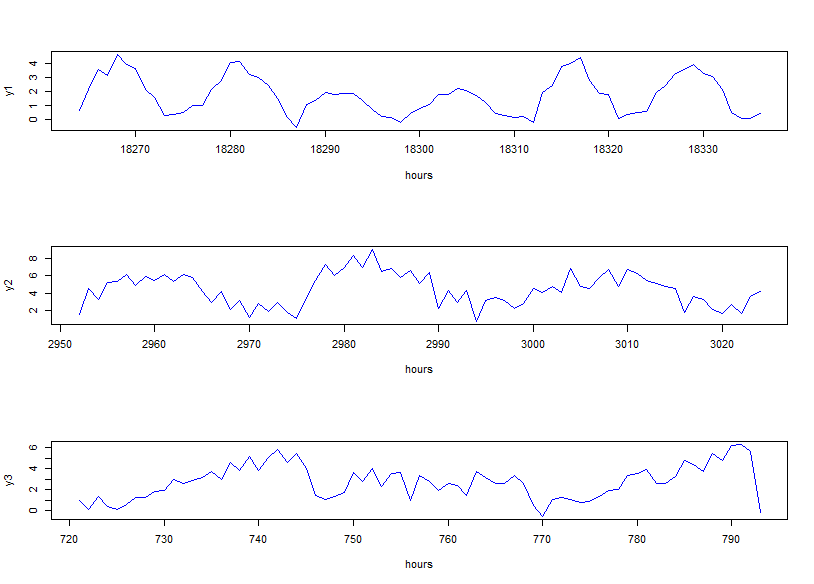
\includegraphics[scale=0.6]{Figures/Anomalies}
	\decoRule
	\caption[Synthetic Anomalies]{Synthetic Anomalies \parencite{own}}
	\label{fig:anomalies}
\end{figure}

For the supervised learning approach the dataset was also labelled. In each case the whole day was marked as an anomaly. In total 30 anomalous days were embedded into the dataset, this corresponds to 1.5 percent of anomalous datapoints.

\subsubsection{Neural Networks}
In the first experiment, a CNN was tested against a RNN in a supervised and also in an unsupervised fashion. As RNN, the type GRU was chosen. As some first attempts showed, that it showed sufficient results with improved computation time compared to the more complex LSTM. 

For the supervised learning approach, the chosen architecture can be seen in table \ref{Tab:Supervised Learning}. As activation function "ReLu" was used. 

\begin{table}[h]
\caption{Supervised Learning}
	\begin{center}
		\begin{tabular}{ | c | c | c | c |}
			\hline
			\thead{} & \thead{Input} & \thead{NN-Architecture} & \thead{Output} \\
			\hline
			\thead{CNN} &  120 past datapoints  & \makecell{2 1D-Convolutional Layers \\ 2 Max-Pooling Layers \\ 1 Dense Layer}  & \makecell{1 Dense Layer \\ with Sigmoid Activation}   \\
			\hline
			\thead{RNN} &  120 past datapoints  & \makecell{2 GRU Layers \\ 1 Dense Layer}  & \makecell{1 Dense Layer \\ with Sigmoid Activation}  \\
			\hline
		\end{tabular}
		\label{Tab:Supervised Learning}
	\end{center}
\end{table}

The used optimizer was Adam, with all its default values. As loss function, the typical binary crossentropy was applied. 
The architecture used for the unsupervised learning approach, displayed in table \ref{Tab:Unupervised Learning}, looked very similar. The main difference between the two architectures was that the CNN was not built as a sequential model. Instead of having one output layer, the CNN has five parallel output layers, each predicting a time series \footnote{More detailed summaries of the models can be found in appendix \ref{AppendixA}}.     

\begin{table}[h]
	\caption{Unupervised Learning}
	\begin{center}
		\begin{tabular}{ | c | c | c | c |}
			\hline
			\thead{} & \thead{Input} & \thead{NN-Architecture} & \thead{Output} \\
			\hline
			\thead{CNN} &  120 past datapoints  & \makecell{2 1D-Convolutional Layers \\ 2 Max-Pooling Layers }  & \makecell{ 5 Dense Layers with \\ 1 regression outputs}   \\
			\hline
			\thead{RNN} &  120 past datapoints  & \makecell{2 GRU Layers}  & \makecell{ 1 Dense Layers with \\ 5 regression outputs}  \\
			\hline
		\end{tabular}
	\label{Tab:Unupervised Learning}
	\end{center}
\end{table}

\subsubsection{Results}


\subsection{Experiment 2}

\subsection{Experiment 3}
